\chapter{Results}

    \todo[inline]{Update with final values}

    \section{Code vs prose task}

        Our top-performing classifier yields a LORO-CV score of: $$0.614$$ (mean), $$0.089$$ (std).\todo[inline]{Exclude bad subjects from training}

        The following is the performance statistics for our model trained on 5 second windows. It from all subjects except one, which is excluded from training and used in testing:

        \begin{verbatim}
        INFO: {
            'precision': 0.7473868367437329, 
            'recall': 0.696405129166862, 
            'fbeta': 0.6703482474923927, 
            'support': array([308, 277]), 
            'bac': 0.696405129166862, 
            'confusion_matrix': array([[141, 167], [ 18, 259]])
        }
        \end{verbatim}

        The following are the performance statistics for our model on the epoch-level. We achieve epoch-level classification by training on 5 second windows which are aggregated into epochs by taking the mean of the prediction probabilities. The same subject selection as the previous statistics is used:

        \begin{verbatim}
        INFO: {
            'precision': 0.8541666666666667, 
            'recall': 0.7666666666666666, 
            'fbeta': 0.7624602332979852, 
            'support': array([15, 17]), 
            'bac': 0.7666666666666666, 
            'confusion_matrix': array([[ 8,  7], [ 0, 17]])
        }
        \end{verbatim}

        \todo[inline]{Use LORO instead of testing subject}
        \begin{table}
            \begin{center}
                \begin{tabular}{ l | c | c }
                  \toprule
                  & Epoch-level (subject \#6) & Window-level (subject \#6) \\ \midrule
                  Precision & 85.4\% & 74.7\% \\
                  Recall & 76.7\% & 69.6\% \\
                  BAC & 76.7\% & 69.6\% \\
                  \bottomrule
                  
                \end{tabular}
                \caption{Performance statistics of our models trained on all subjects except subject number \#6 which is used for testing}\label{fig:stats}
            \end{center}
        \end{table}

        \begin{figure}[h]
        \centering
        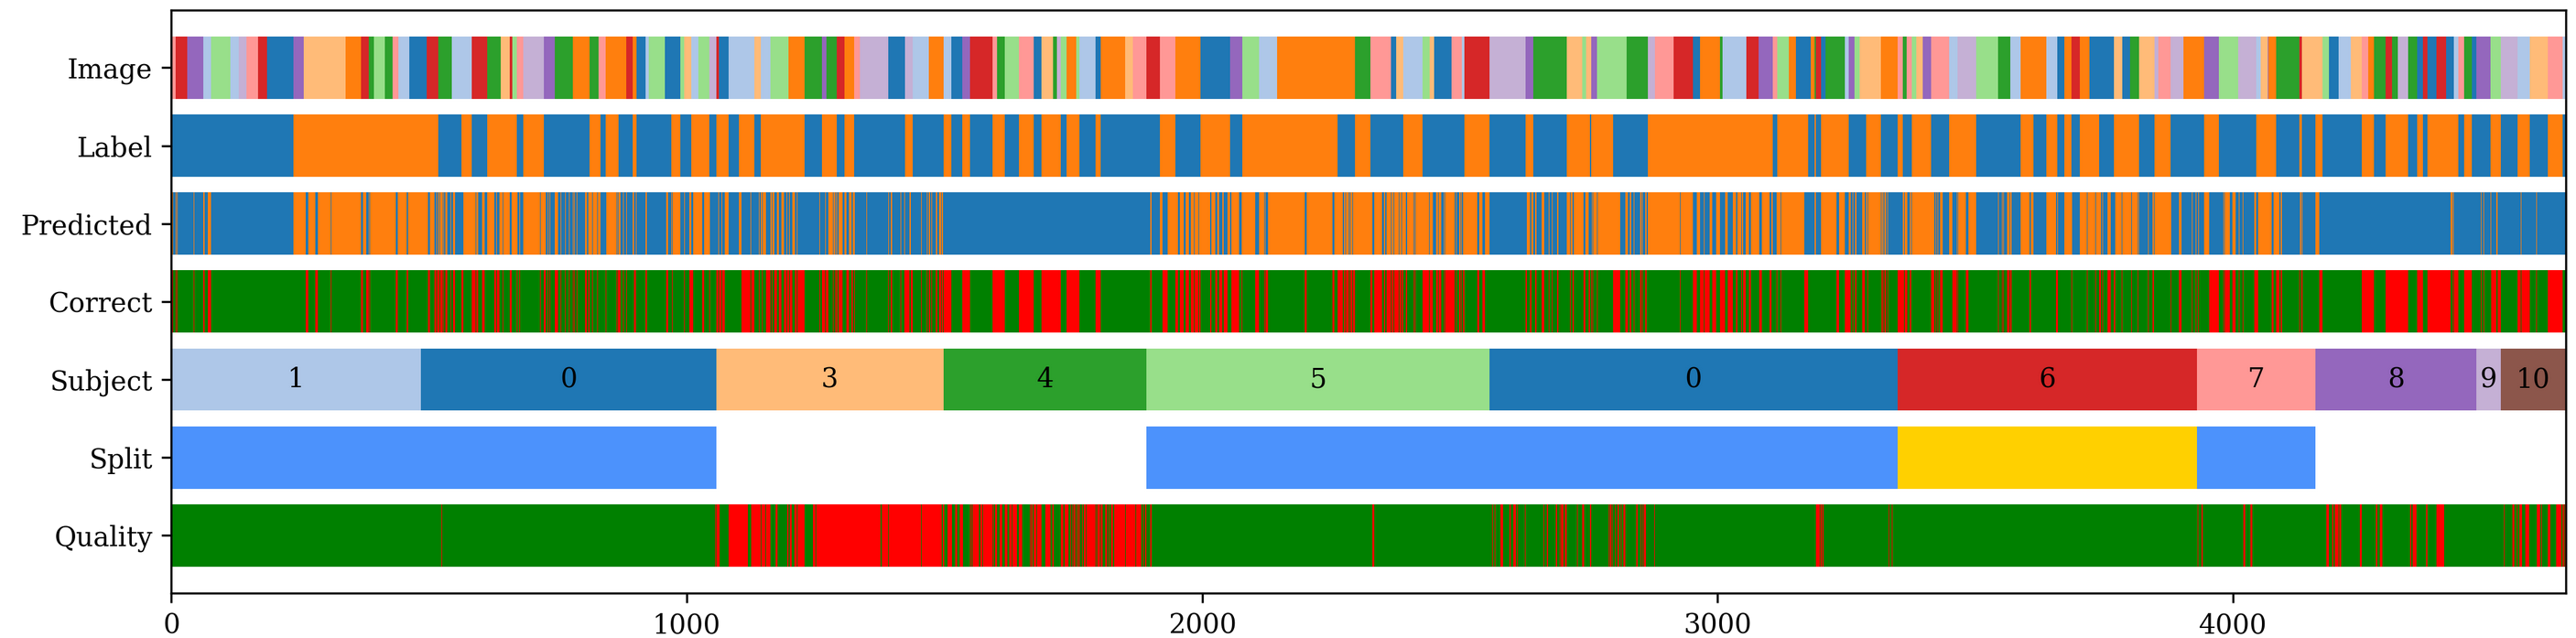
\includegraphics[width=16cm]{img/timebars.png}
        \caption{A visualization of the labeled data, the predicted class, the subject, the training and testing split, and a measure of signal quality.}\label{fig:timebars}
        \end{figure}

        Our classifier performance is\ldots

        \begin{figure}[h]
        \centering
        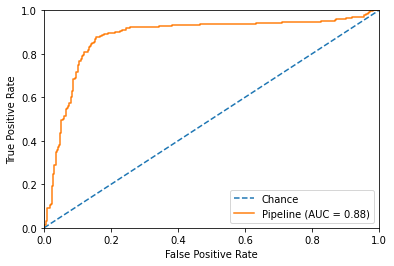
\includegraphics[width=12cm]{img/roccurve.png}
        \caption{Receiver operating characteristic (ROC) curve}\label{fig:roc}
        \end{figure}


        Compared to Fucci\ldots

    \section{Naturalistic device activity}

        Our classifier performance is\ldots

